\documentclass{article}

%----
%  Colin Tan
%  Basic setup for homework
%----
%----------------------------------------------------------------------------------------
%	PACKAGES AND OTHER DOCUMENT CONFIGURATIONS
%----------------------------------------------------------------------------------------

\usepackage{fancyhdr} % Required for custom headers
\usepackage{lastpage} % Required to determine the last page for the footer
\usepackage{extramarks} % Required for headers and footers
\usepackage{graphicx} % Required to insert images

\usepackage{listings} % listing codes

\usepackage{siunitx} % SI units
\usepackage{amsmath, amssymb} % Math

\usepackage{tikz} % Drawing graphs
\usepackage{pgfplots} % Drawing mathematical plots
\usepgfplotslibrary{fillbetween}
\pgfplotsset{compat=1.10} % pgf compatable version
\usepackage{float} % Flotation control

\usepackage{framed} % Framing answers
\usepackage{enumitem} % Customize enumeration style

\usepackage{multicol} % Required for columizing
\usepackage{caption} % For non-numbered captions
\usepackage{subcaption} % for caption of subfigures

\usepackage[us]{datetime} % Print date in US format

% Margins
\topmargin=-0.45in
\evensidemargin=0in
\oddsidemargin=0in
\textwidth=6.5in
\textheight=9.0in
\headsep=0.25in 

\linespread{1.1} % Line spacing

% Set up the header and footer
\pagestyle{fancy}
\lhead{\hmwkAuthorName} % Top left header
\chead{\hmwkClass\ (\hmwkClassInstructor\ \hmwkClassTime): \hmwkTitle} % Top center header
\rhead{\firstxmark} % Top right header
\lfoot{\lastxmark} % Bottom left footer
\cfoot{} % Bottom center footer
\rfoot{Page\ \thepage\ of\ \pageref{LastPage}} % Bottom right footer
\renewcommand\headrulewidth{0.4pt} % Size of the header rule
\renewcommand\footrulewidth{0.4pt} % Size of the footer rule

\setlength\parindent{0pt} % Removes all indentation from paragraphs

%----------------------------------------------------------------------------------------
%	DOCUMENT STRUCTURE COMMANDS
%----------------------------------------------------------------------------------------

% Header and footer for when a page split occurs within a problem environment
\newcommand{\enterProblemHeader}[1]{
	\nobreak\extramarks{#1}{#1 continued on next page\ldots}\nobreak
	\nobreak\extramarks{#1 (continued)}{#1 continued on next page\ldots}\nobreak
}

% Header and footer for when a page split occurs between problem environments
\newcommand{\exitProblemHeader}[1]{
	\nobreak\extramarks{#1 (continued)}{#1 continued on next page\ldots}\nobreak
	\nobreak\extramarks{#1}{}\nobreak
}

\setcounter{secnumdepth}{0} % Removes default section numbers
\newcounter{homeworkProblemCounter} % Creates a counter to keep track of the number of problems

\newcommand{\homeworkProblemName}{}
\newenvironment{homeworkProblem}[1][Problem \arabic{homeworkProblemCounter}]{ % Makes a new environment called homeworkProblem which takes 1 argument (custom name) but the default is "Problem #"
	\stepcounter{homeworkProblemCounter} % Increase counter for number of problems
	\renewcommand{\homeworkProblemName}{#1} % Assign \homeworkProblemName the name of the problem
	\section{\homeworkProblemName} % Make a section in the document with the custom problem count
	\enterProblemHeader{\homeworkProblemName} % Header and footer within the environment
}{
	\exitProblemHeader{\homeworkProblemName} % Header and footer after the environment
}

\newcommand{\problemAnswer}[1]{ % Defines the problem answer command with the content as the only argument
	\noindent\begin{oframed}
		#1
	\end{oframed}
}

\newcommand{\homeworkSectionName}{}
\newenvironment{homeworkSection}[1]{ % New environment for sections within homework problems, takes 1 argument - the name of the section
	\renewcommand{\homeworkSectionName}{#1} % Assign \homeworkSectionName to the name of the section from the environment argument
	\subsection{\homeworkSectionName} % Make a subsection with the custom name of the subsection
	\enterProblemHeader{\homeworkProblemName\ [\homeworkSectionName]} % Header and footer within the environment
}{
	\enterProblemHeader{\homeworkProblemName} % Header and footer after the environment
}

%----------------------------------------------------------------------------------------
%	TITLE PAGE
%----------------------------------------------------------------------------------------

\title{
\vspace{2in}
\textmd{\textbf{\hmwkClass:\ \hmwkTitle}}\\
\normalsize\vspace{0.1in}\small{Due\ on\ \hmwkDueDate}\\
\vspace{0.1in}\large{\textit{\hmwkClassInstructor\ \hmwkClassTime}}
\vspace{3in}
}

\author{\textbf{\hmwkAuthorName}}
\date{\today} % Insert date here if you want it to appear below your name

\usetikzlibrary{shapes.geometric, calc}
\DeclareSIUnit\c{\mathit{c}}
%\everymath{\displaystyle}
%----------------------------------------------------------------------------------------
%	NAME AND CLASS SECTION
%----------------------------------------------------------------------------------------

\newdate{DueDate}{15}{04}{2015} % Due date in {dd}{mm}{yyyy}
\newcommand{\hmwkTitle}{Homework\ 9} % Assignment title
\newcommand{\hmwkDueDate}{\dayofweekname{\getdateday{DueDate}}{\getdatemonth{DueDate}}{\getdateyear{DueDate}} \displaydate{DueDate}} % Due date
\newcommand{\hmwkClass}{PHYS\ 161} % Course/class
\newcommand{\hmwkClassTime}{11:00am} % Class/lecture time
\newcommand{\hmwkClassInstructor}{Professor Landee} % Teacher/lecturer
\newcommand{\hmwkAuthorName}{Zhuoming Tan} % Your name

%----------------------------------------------------------------------------------------

\begin{document}

\maketitle
\newpage
%----------------------------------------------------------------------------------------
%	TABLE OF CONTENTS
%----------------------------------------------------------------------------------------

%\setcounter{tocdepth}{1} % Uncomment this line if you don't want subsections listed in the ToC

%\newpage
%\tableofcontents
%\newpage

%----------------------------------------------------------------------------------------
%	PROBLEM 1
%----------------------------------------------------------------------------------------

% To have just one problem per page, simply put a \clearpage after each problem

\begin{homeworkProblem}
	(9.1) \textit{The missing term}

	Due to the contradiction between Eqs.~(9.2) and (9.5), we know that there must be an extra term in the $\nabla\times\mathbf{B}$ relation, as we found in Eq.~(9.10). Call this term $\mathbf{W}$. In the text, we used the Lorentz transformations to motivate a guess for $\mathbf{W}$. Find $\mathbf{W}$ here by taking the divergence of both sides of $\nabla\times\mathbf{B}=\mu_0\mathbf{J}+\mathbf{W}$. Assume that the only facts you are allowed to work with are (1) $\nabla\cdot\mathbf{E}=\rho/\epsilon_0$, (2) $\nabla\cdot\mathbf{B}=0$, (3) $\nabla\cdot\mathbf{J}=-\partial\rho/\partial t$, and (4) $\nabla\times\mathbf{B}=\mu_0\mathbf{J}$ in the case of steady currents.
	% Question

	\textbf{Solution}
	\begin{align*}
		\nabla\times\mathbf{B}&=\mu_0\mathbf{J}+\mathbf{W} \\
		\nabla\cdot\left(\nabla\times\mathbf{B}\right)&=\nabla\cdot\left(\mu_0\mathbf{J}+\mathbf{W}\right) \\
		0&=\mu_0\nabla\cdot\mathbf{J}+\nabla\cdot\mathbf{W} \\
		\nabla\cdot\mathbf{W}&=-\mu_0\nabla\cdot\mathbf{J} \\
		\nabla\cdot\mathbf{W}&=\mu_0\frac{\partial\rho}{\partial t} \\
		\nabla\cdot\mathbf{W}&=\mu_0\epsilon_0\frac{\partial}{\partial t}\nabla\cdot\mathbf{E} \\
		\mathbf{W}&=\mu_0\epsilon_0\frac{\partial}{\partial t}\mathbf{E} \\
	\end{align*}
\end{homeworkProblem}

%----------------------------------------------------------------------------------------
%	PROBLEM 2
%----------------------------------------------------------------------------------------

\begin{homeworkProblem}
	(9.3) \textit{A charge and a half-infinite wire}

	A half-infinite wire carries current $I$ from negative infinity to the origin, where it builds up at a point charge with increasing $q$ (so $dq/dt=I$). Consider the circle shown in Fig.~\ref{fig:wire}, which has radius $b$ and subtends an angle $2\theta$ with respect to the charge. Calculate the integral $\int\mathbf{B}\cdot d\mathbf{s}$ around this circle. Do this in three ways.
	\begin{figure}[H]
		\centering
		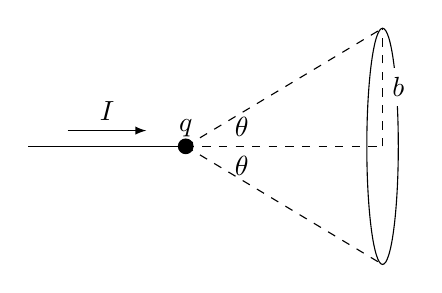
\begin{tikzpicture}
			\draw (0, 0) ellipse (0.2 and 1.5);
			\draw[dashed] (-2.5, 0) -- (0, 0);
			\draw[dashed] (-2.5, 0) -- (0, 1.5);
			\draw[dashed] (-2.5, 0) -- (0, -1.5);
			\draw[dashed] (0, 0) -- (0, 1.5) node[midway, right, fill = white] {$b$};
			\fill (-2.5, 0) circle[radius = 0.1] node[above] {$q$};
			\draw (-4.5, 0) -- (-2.5, 0);
			\draw[-latex] (-4, 0.2) -- (-3, 0.2) node[midway, above] {$I$};
			\node[anchor = south west] at (-2, 0) {$\theta$};
			\node[anchor = north west] at (-2, 0) {$\theta$};
		\end{tikzpicture}
		\caption{}\label{fig:wire}
	\end{figure}
	\begin{enumerate}[label= (\alph*)]
		\item Find the $\mathbf{B}$ field at a given point on the circle by using the Biot-Savart law to add up the contributions from the different parts of the wire.
		\begin{item}
			Use the integrated form of Maxwell's equation (that is, the generalized form of Amp\`{e}re's law including the displacement current),
			\begin{equation}\tag{9.59}
				\int_C\mathbf{B}\cdot d\mathbf{s}=\mu_0 I+\mu_0\epsilon_0\int_S\frac{\partial\mathbf{E}}{\partial t}\cdot d\mathbf{a}
			\end{equation}
			with $S$ chosen to be a surface that is bounded by the circle and doesn't intersect the wire, but is otherwise arbitrary. (You can invoke the result from Problem 1.15.)
		\end{item}
		\item Use the same strategy as in (b), but now let $S$ intersect the wire.
	\end{enumerate}
	% Question

	\textbf{Solution}
	\begin{enumerate}[label= (\alph*)]
		\begin{item}
			For a point $P$ on the circle, let the angle between verticle direction and the line connecting $P$ and points on the wire be $\phi$. By BSL
			\[
				B=\frac{\mu_0I}{4\pi}\int_\theta^{\pi/2}\frac{\cos\phi}{r^2}\,dl=\frac{\mu_0I}{4\pi b}(1-\cos\theta)
			\]
			tangential to the circle. So
			\[
				\int_C\mathbf{B}\cdot d\mathbf{s}=2\pi b\frac{\mu_0I}{4\pi b}(1-\cos\theta)=\frac{\mu_0I}{2}(1-\cos\theta)
			\]
		\end{item}
		\begin{item}
			$\mu_0I=0$ becuase the surface chosen does not intersect with the wire. From Problem 1.15, flux of field through the circle is
			\[
				\Phi_E=\frac{q}{2\epsilon_0}(1-\cos\theta)
			\]
			so
			\[
				\mu_0\epsilon_0\int_S\frac{\partial\mathbf{E}}{\partial t}\cdot d\mathbf{a}=\mu_0\epsilon_0\frac{\partial}{\partial t}\int_S\mathbf{E}\cdot d\mathbf{a}=\mu_0\epsilon_0\frac{\partial\Phi_E}{\partial t}=\frac{\mu_0I}{2}(1-\cos\theta)
			\]
		\end{item}
		\begin{item}
			Include $\mu_0I$ now. Consider a cone-like shape that encloses the charge. The base would be the surface examined in part (b), and the side will be the one we are about to look at right now. ${\Phi_E}'=q/\epsilon_0-\Phi_E$. So
			\[
				\mu_0I+\mu_0\epsilon_0\int_S\frac{\partial\mathbf{E}}{\partial t}\cdot d\mathbf{a}=\mu_0I+\mu_0\epsilon_0\frac{\partial{\Phi_E}'}{\partial t}=\frac{\mu_0I}{2}(1-\cos\theta)
			\]
		\end{item}
	\end{enumerate}
\end{homeworkProblem}

%----------------------------------------------------------------------------------------
%	PROBLEM 3
%----------------------------------------------------------------------------------------

\begin{homeworkProblem}
	(9.5) \textit{Maxwell's equations for a moving charge}\ldots (problem omitted)
	% Question

	\textbf{Solution}
	\begin{equation}\tag{5.13}
		E'=\frac{Q}{4\pi\epsilon_0{r'}^2}\frac{1-\beta^2}{{(1-\beta^2\sin^2\theta')}^{3/2}}
	\end{equation}
	\begin{enumerate}[label = (\alph*)]
		\begin{item}
			So
			\begin{align*}
				\nabla\cdot\mathbf{B}&=\frac{1}{c^2}\nabla\cdot(\mathbf{v}\times\mathbf{E}) \\
				&=\frac{1}{c^2}\left[\mathbf{E}\cdot(\nabla\times\mathbf{v})-\mathbf{v}\cdot(\nabla\times\mathbf{E})\right]
			\end{align*}
			And $\nabla\times\mathbf{v}=0$ because $\mathbf{v}$ is constant. $\nabla\times\mathbf{E}$ is perpendicular to $\mathbf{v}$, making their dot products zero as well. So $\nabla\cdot\mathbf{B}=0$.
		\end{item}
		\begin{item}
			From 5.13, with
			\[
				D={(\gamma x)}^2+y^2+z^2
			\]
			the field becomes
			\[
				\mathbf{E}=\frac{\gamma Q}{4\pi\epsilon_0D^{3/2}}(x,y,z)
			\]
			So
			\[
				{(\nabla\times\mathbf{E})}_y=\frac{\gamma Q}{4\pi\epsilon_0}\left(\frac{-3xz}{D^{5/2}}+\frac{3\gamma^2xz}{D^{5/2}}\right)=\frac{\gamma Q}{4\pi\epsilon_0}\frac{3\gamma^2v^2xz}{c^2D^{5/2}}\hat{\mathbf{y}}
			\]
			and the other components are zero.
			\[
				\frac{\partial\mathbf{B}}{\partial t}=\frac{1}{c^2}\frac{\partial}{\partial t}(\mathbf{v}\times\mathbf{E})=\frac{1}{c^2}\mathbf{v}\times\frac{\partial\mathbf{E}}{\partial t}
			\]
			Compute
			\[
				\frac{\partial E_z}{\partial t}=\frac{\gamma Q}{4\pi\epsilon_0}\frac{3\gamma^2xzv}{D^{5/2}}
			\]
			\[
				\frac{\partial\mathbf{B}}{\partial t}=\frac{v}{c^2}\hat{\mathbf{x}}\times\frac{\gamma Q}{4\pi\epsilon_0}\frac{3\gamma^2xzv}{D^{5/2}}\hat{\mathbf{z}}=-\nabla\times\mathbf{E}
			\]
		\end{item}
	\end{enumerate}
\end{homeworkProblem}

%----------------------------------------------------------------------------------------
%	PROBLEM 4
%----------------------------------------------------------------------------------------

\begin{homeworkProblem}
	(9.10) \textit{Energy flow from a wire}\ldots (problem omitted)
	% Question

	\textbf{Solution}
	
	For the wire being considered as a tube, its magnetic field is
	\[
		B=\frac{\mu_0I}{2\pi b}
	\]
	tangential to the wire. On the other hand for the sphere, its $E$ field is radial
	\[
		E=\frac{Q}{4\pi\epsilon_0r^2}
	\]
	So Poynting vector
	\[
		S=\frac{EB}{\mu_0}=\frac{QI}{4\pi\epsilon_0r^2\times2\pi b}
	\]
	Integrate this over the surface of the tube, on which $da=2\pi b\,dr$
	\[
		\int S\,da=\int_R^\infty\frac{QI}{4\pi\epsilon_0r^2\times2\pi b}2\pi b\,dr=\frac{d}{dt}\frac{Q^2}{8\pi\epsilon_0R}
	\]
	To see energy stored in the electric field of the sphere, constant $\phi=Q/4\pi\epsilon_0R$
	\[
		U=\frac{1}{2}\int\rho\phi{\,}dv=\frac{1}{2}\phi\int\rho{\,}dv=\frac{1}{2}\frac{Q}{4\pi\epsilon_0R}Q=\frac{Q^2}{8\pi\epsilon_0R}
	\]
	Therefore energy flow is equal to the energy stored.
\end{homeworkProblem}

%----------------------------------------------------------------------------------------
%	PROBLEM 5
%----------------------------------------------------------------------------------------

\begin{homeworkProblem}
	(9.14) \textit{Sphere with a hole}\ldots (problem omitted)
	% Question

	\textbf{Solution}

	Integral over the circumference $C$ is
	\[
		\int_C\mathbf{B}\cdot d\mathbf{s}=\mu_0I
	\]
	And integral over the surface $S$ is
	\[
		\int_S\left(\mu_0\epsilon_0\frac{\partial\mathbf{E}}{\partial t}+\mu_0\mathbf{J}\right)\cdot d\mathbf{a}
	\]
	but the wire goes through the hole, so $\mathbf{J}=0$. Therefore, becuase the charge $Q(t)=It$, and $E=\frac{Q}{4\pi\epsilon_0r^2}$,
	\[
		\mu_0\epsilon_0\frac{\partial}{\partial t}\int_S\mathbf{E}\cdot d\mathbf{a}=\mu_0\epsilon_0\frac{\partial}{\partial t}\left(\frac{It}{4\pi\epsilon_0r^2}\cdot4\pi r^2\right)=\mu_0I
	\]
	Therefore the integral form of Maxwell's equation is satisfied.
\end{homeworkProblem}

%----------------------------------------------------------------------------------------
%	PROBLEM 6
%----------------------------------------------------------------------------------------

\begin{homeworkProblem}
	(9.15) \textit{Field inside a discharging capacitor}\ldots (problem omitted)
	% Question

	\textbf{Solution}

	Imagine a circle $C$ centered with the direction of the wire, with radius $r$, so that $P$ lies on the circle. If the magnetic field $B$ is constant,
	\[
		\int_C\mathbf{B}\cdot d\mathbf{s}=2\pi rB
	\]
	On the other hand, no current passes through the circle, for which $\mathbf{J}=0$. $\mathbf{E}=\frac{\sigma}{\epsilon_0}=\frac{Q}{\pi b^2\epsilon_0}$. $a=2\pi b^2$.
	\[
		\int_S\left(\mu_0\epsilon_0\frac{\partial\mathbf{E}}{\partial t}+\mu_0\mathbf{J}\right)\cdot d\mathbf{a}=\mu_0\epsilon_0\int_S\frac{\partial\mathbf{E}}{\partial t}\cdot d\mathbf{a}=\mu_0\epsilon_0\int_S\frac{\mathbf{I}}{\pi b^2\epsilon_0}\cdot d\mathbf{a}=\frac{\mu_0r^2I}{b^2}
	\]
	Therefore $2\pi rB=\frac{\mu_0r^2I}{b^2}$, or $B=\frac{\mu_0Ir}{2\pi b^2}$.
\end{homeworkProblem}

%----------------------------------------------------------------------------------------
%	PROBLEM 7
%----------------------------------------------------------------------------------------

\begin{homeworkProblem}
	(9.20) \textit{Kicked by a wave}\ldots (problem omitted)
	% Question

	\textbf{Solution}
	\begin{equation}\tag{9.28}
		\mathbf{E}=\frac{E_0\hat{\mathbf{y}}}{1+\frac{{(x+ct)}^2}{l^2}},\quad\mathbf{B}=\frac{-(E_0/c)\hat{\mathbf{z}}}{1+\frac{{(x+ct)}^2}{l^2}}
	\end{equation}
	The change in momentum, when $x$ as well as $B$ is negligible
	\[
		\Delta\mathbf{p}=\int\mathbf{F}\,dt=e\hat{\mathbf{y}}\times\SI{100}{\kilo\volt\per\m}\int_{-\infty}^\infty\frac{dt}{1+\frac{{(ct)}^2}{l^2}}=\frac{e\pi l}{c}\hat{\mathbf{y}}\times\SI{100}{\kilo\volt\per\m}
	\]
	So velocity
	\[
		v=\frac{p}{m}=\frac{e\pi l}{mc}\hat{\mathbf{y}}\times\SI{100}{\kilo\volt\per\m}
	\]
	So position
	\[
		s=vt=\frac{e\pi l}{mc}\hat{\mathbf{y}}\times\SI{1e5}{\volt\per\m}\times\SI{1e-6}{\s}\approx0.10l\hat{\mathbf{y}}
	\]
\end{homeworkProblem}

%----------------------------------------------------------------------------------------
%	PROBLEM 8
%----------------------------------------------------------------------------------------

\begin{homeworkProblem}
	(9.22) \textit{Plane-wave pulse}\ldots (problem omitted)
	% Question

	\textbf{Solution}
	\begin{enumerate}[label = (\alph*)]
		\begin{item}
			Use Amp\`{e}re's law
			\[
				\oint\mathbf{B}\cdot d\mathbf{l}=\int_S\left(\mu_0\epsilon_0\frac{\partial\mathbf{E}}{\partial t}+\mu_0\mathbf{J}\right)\cdot d\mathbf{a}
			\]
			Only the section inside the slab contributes to the integral
			\[
				\oint\mathbf{B}\cdot d\mathbf{l}=Bl
			\]
			and
			\[
				\int_S\left(\mu_0\epsilon_0\frac{\partial\mathbf{E}}{\partial t}+\mu_0\mathbf{J}\right)\cdot d\mathbf{a}=\mu_0\epsilon_0\frac{\partial}{\partial t}\int_S\mathbf{E}\cdot d\mathbf{a}=\mu_0\epsilon_0\frac{\partial\Phi_E}{\partial t}=\mu_0\epsilon_0 vEl
			\]
			So $c^2B=vE$.
		\end{item}
		\begin{item}
			Use Faraday's law
			\[
				\oint\mathbf{E}\cdot d\mathbf{s}=-\frac{d\Phi_B}{dt}
			\]
			This time let the loop be into the page, perpendicular to $\mathbf{B}$. Normal vector points upward.
			\[
				-\frac{d\Phi_B}{dt}=Bvl
			\]
			\[
				\oint\mathbf{E}\cdot d\mathbf{s}=El
			\]
			So $E=Bv$
		\end{item}
	\end{enumerate}
	After all $v=c$.
\end{homeworkProblem}

%----------------------------------------------------------------------------------------
%	PROBLEM 9
%----------------------------------------------------------------------------------------

\begin{homeworkProblem}
	(9.30) \textit{Comparing the energy densities}

	Consider the capacitor example in Section 9.6.2, but now let the current change in a way that makes the electric field inside the capacitor take the form of $E(t)=E_0\cos\omega t$. The induced magnetic field is given in Eq.~(9.46). Show that the energy density of the magnetic field is much smaller than the energy density of the electric field, provided that the time scale of $\omega$ (namely $2\pi/\omega$) is much longer than the time it takes light to travel across the diameter of the capacitor disks. (As in Problem 9.6, we are ignoring higher-order effects.)
	% Question

	\textbf{Solution}
	\[
		B=\frac{\mu_0\epsilon_0r}{2}\frac{\partial E}{\partial t}=-\frac{\mu_0\epsilon_0r}{2}E_0\sin\omega t
	\]
\end{homeworkProblem}

%----------------------------------------------------------------------------------------
%	PROBLEM 10
%----------------------------------------------------------------------------------------

\begin{homeworkProblem}
	(9.32) \textit{A Lorentz invariant}\ldots (problem omitted)
	% Question

	\textbf{Solution}
\end{homeworkProblem}
%----------------------------------------------------------------------------------------

\end{document}
